 \documentclass[25pt, a0paper, portrait, margin=0mm, innermargin=15mm,
     blockverticalspace=10mm, colspace=15mm, subcolspace=8mm]{tikzposter}

% --------------
% FONT
% --------------

% Change font: https://www.overleaf.com/learn/latex/Font_typefaces
\usepackage[T1]{fontenc}
\usepackage{tgbonum}
\usepackage{lmodern} %mix italic and bold

% increase tikzfigure caption  font size
\renewenvironment{tikzfigure}[1][]{
  \def \rememberparameter{#1}
  \vspace{10pt}
  \refstepcounter{figurecounter}
  \begin{center}
  }{
    \ifx\rememberparameter\@empty
    \else %nothing
    \\[10pt]
    {\Large Fig.~\thefigurecounter: \rememberparameter}
    \fi
  \end{center}
}

\usepackage[none]{hyphenat} % avoid hyphenation

% % --------------
% % COLORS
% % --------------
\definecolor{mydarkblue}{RGB}{115,172,255}
\definecolor{mylightblue}{RGB}{204,233,239}
% colors for 4 offspring groups
\definecolor{myyellow}{RGB}{255,230,128}
\definecolor{myorange}{RGB}{255,102,0}
\definecolor{myblue}{RGB}{170,204,255}
\definecolor{mypurple}{RGB}{170,0,212}

% -------------
% THEME SETTING
% -------------
\usetheme{Autumn}
\colorlet{titlebgcolor}{mydarkblue}
\colorlet{titlefgcolor}{black}
\colorlet{backgroundcolor}{white}

\colorlet{blocktitlebgcolor}{mylightblue}
\colorlet{blockbodybgcolor}{mylightblue}
\colorlet{blocktitlefgcolor}{black}

% -------------------------
% TITLE BLOCK
% -------------------------
\title{\textbf{\parbox{\linewidth}{\centering Parasite infection mediates intergenerational DNA methylation \\ in the three-spined stickleback \textit{(Gasterosteus aculeatus)}}}}
\author{}
\institute{\vspace{-1em}}

% -------------------------
% START
% -------------------------
\begin{document}
\maketitle[titletoblockverticalspace=0mm]
% % add fish picture next to title block
\node[anchor=west] at (TP@title.west) {\includegraphics[width=10cm]{fig/fishFlockL.png}};

-----------------
% AUTHORS BLOCK
% -------------------------
\colorlet{blockbodybgcolor}{white}
\colorlet{blocktitlebgcolor}{white}
% \vspace{-15em}
\block{}{
\begin{center}
\LARGE \textbf{Alice~Balard\textsuperscript{1}}, Kostas~Sagonas\textsuperscript{2}, Joshka~Kaufmann\textsuperscript{3,4}, Melanie~Heckwolf\textsuperscript{5,6}, Christophe Eizaguirre\textsuperscript{1}\\ \LARGE a.balard@qmul.ac.uk 
\includegraphics[width=2.5cm]{fig/twitterlogo.png}@alice\_balard; @EizaguirreLab
\end{center}
\vspace{5mm}
\large \textsuperscript{1}Queen Mary University of London, UK; \textsuperscript{2} National and Kapodistrian University of Athens, Greece; \textsuperscript{3} University College Cork, Ireland; \textsuperscript{4} Marine Institute, Newport, Ireland; \textsuperscript{5} Smithsonian Tropical Research Institute, Panama; \textsuperscript{6} Leibniz Centre for Tropical Marine Research, Germany}
\colorlet{blockbodybgcolor}{mylightblue} % back to default colour

% -------------------------
% INTRO
% -------------------------
\block{}
{\Large
\begin{enumerate}
  \item Paternal infection by the nematode \textit{Camallanus lacustris} is associated with increased selection in offspring but also increased tolerance upon infection\textsuperscript{1}
  \item Genome-wide DNA methylation patterns differ between infected and control fish, demonstrating the link between infection and DNA methylation\textsuperscript{2}
\end{enumerate}
\vspace{5mm} %5mm vertical space
\textbf{Can parental DNA methylation induced by the infection be transmitted to the next generation, and is it an underlying mechanism of the observed phenotypic differences?}
}

% -------------------------
% MATANDMET
% -------------------------

\begin{columns}

  \column{0.6} \block{Material \& methods}{\Large
    \begin{itemize}
      \item Methylome sequencing: \textbf{Reduced Representation Bisulfite Sequencing} single-end reads of 100bp long, Illumina HiSeq 2500. Alignment on a European gynogen genome\textsuperscript{3} and methylation call with BSBolt. Downstream analyses with Methylkit
      \item Positional methylation: 
          \begin{itemize}
          \item \textbf{Is the methylation pattern affected by paternal/offspring treatment?}
          \end{itemize}
      \item Differential methylation: 
          \begin{itemize}
          \item \textbf{Which are the specific differences between paternal/offspring treatment groups?}
          \item \textbf{Can we correlation theses positions with the phenotype?}
          \end{itemize}
      \item \textbf{Link methylation and phenotype}:
        \begin{itemize} 
        \item PCA of methylation values at sites which are differentially methylated in at least 4 out of 8 brother pairs
        \item Extract first and second axes
        \item Linear model of Body condition index explained by:\\ PCA1 * PCA2 * Number of worms * Paternal treatment
        \end{itemize}
    \end{itemize}
 }
 % -------------------------
% RESULTS 1
% -------------------------
\block{1. DNA methylation profiles cluster by genetic background}{ 
  \Large \centering 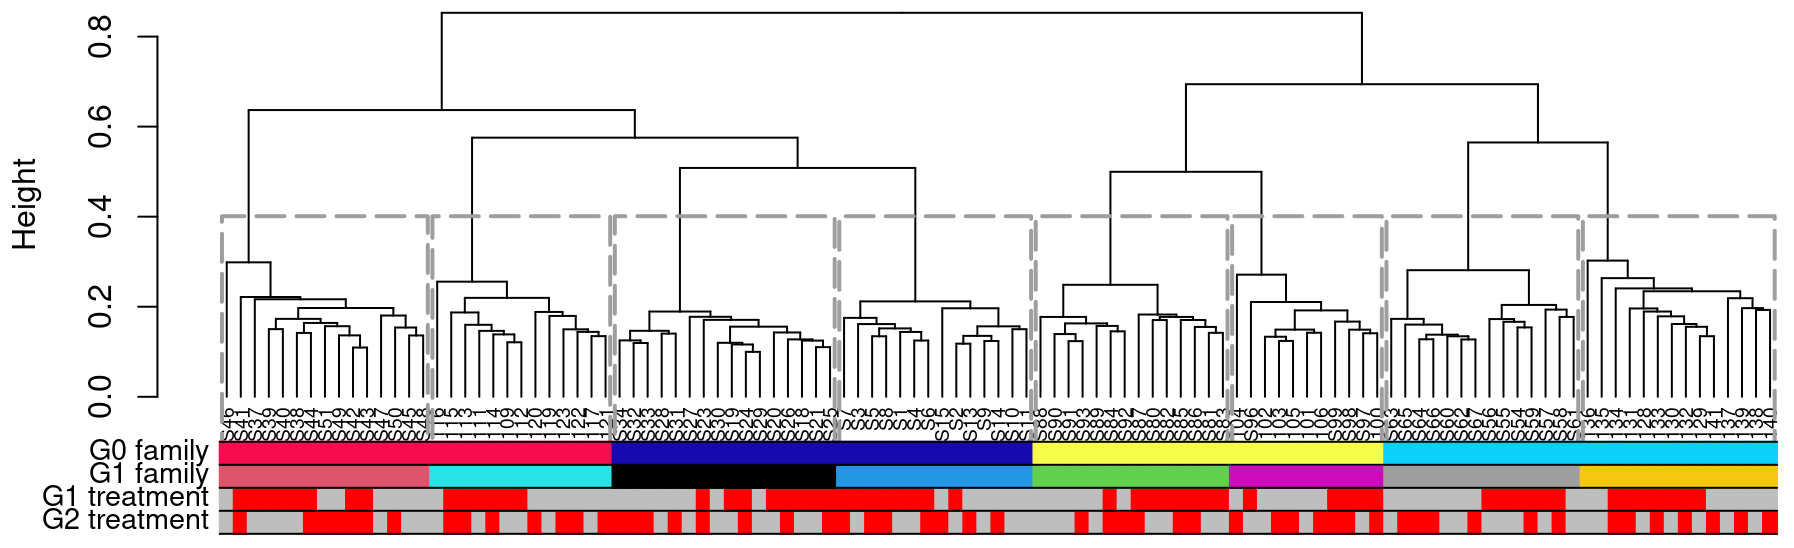
\includegraphics[scale=1.7]{fig/cluster.png}
}
 
 \colorlet{blockbodybgcolor}{white} % set block to white for expe desing
 \column{0.4} \block{}{
               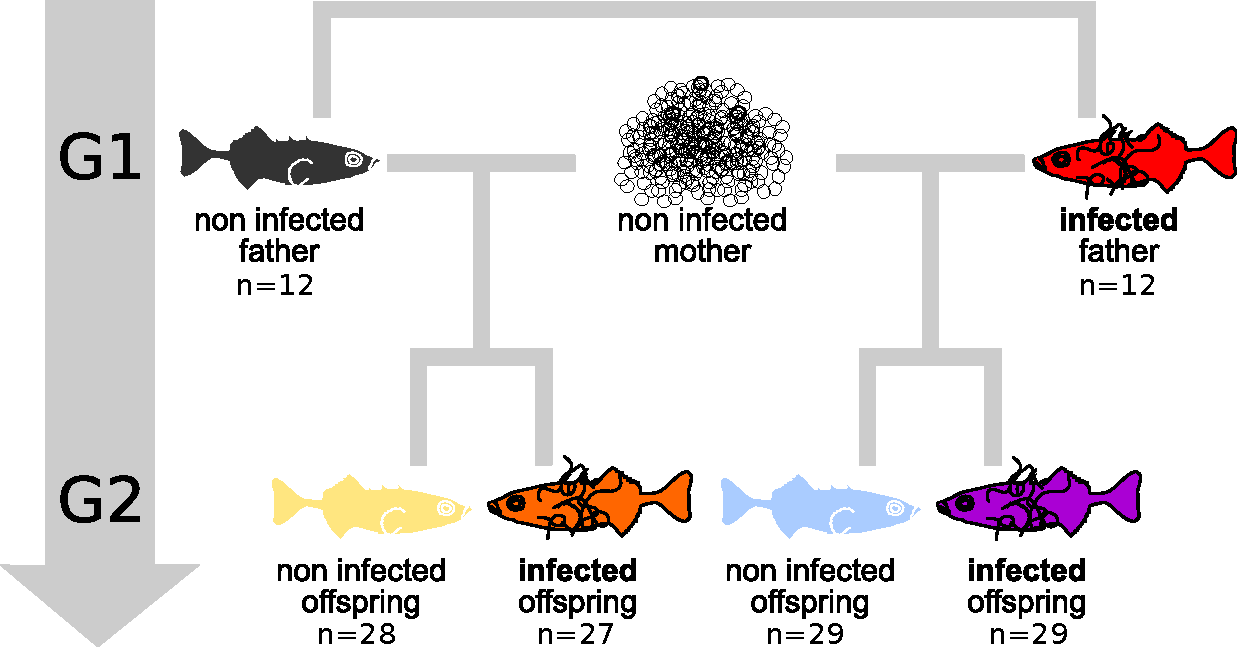
\includegraphics[scale=1.3]{fig/designExpe.pdf}
    }
\colorlet{blockbodybgcolor}{mylightblue} % back to default colour
% -------------------------
% RESULTS 2
% -------------------------
\block{2. Methylation is more affected by the paternal infection than by the offspring infection itself}{
\Large \centering 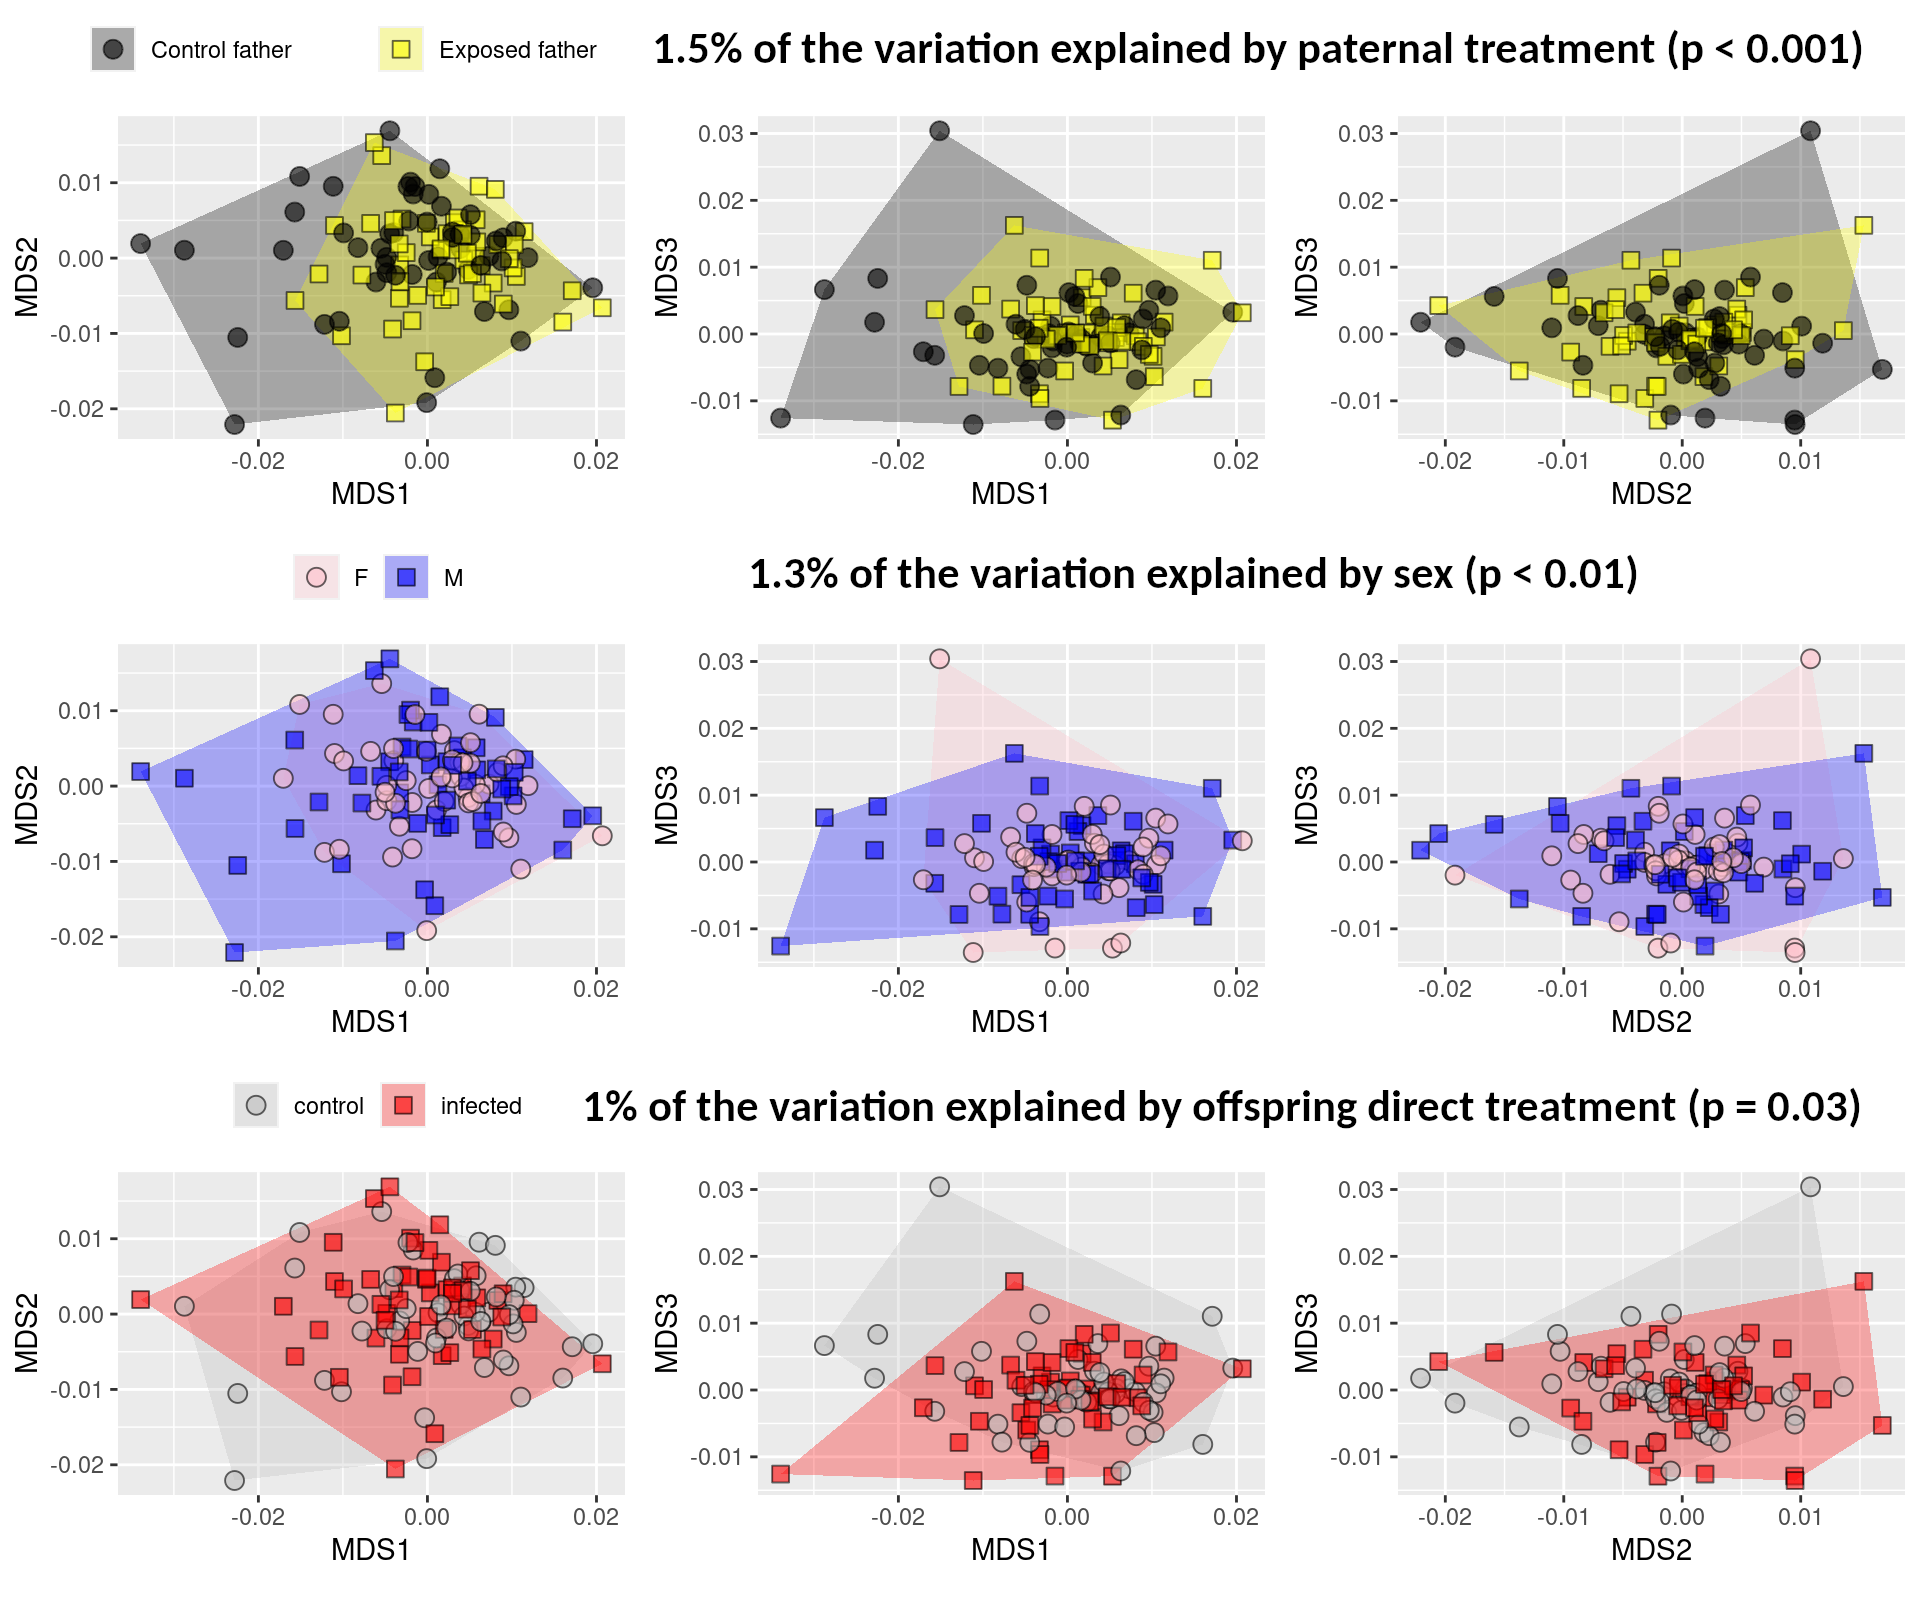
\includegraphics[scale=1]{fig/NMDS.png}}

\end{columns}


\begin{columns}\column{0.56}

% -------------------------
% RESULTS 3
% -------------------------
\block{3. Specific methylated sites linked with paternal infection are associated with genes related to immunity and transcription}{
\Large \centering 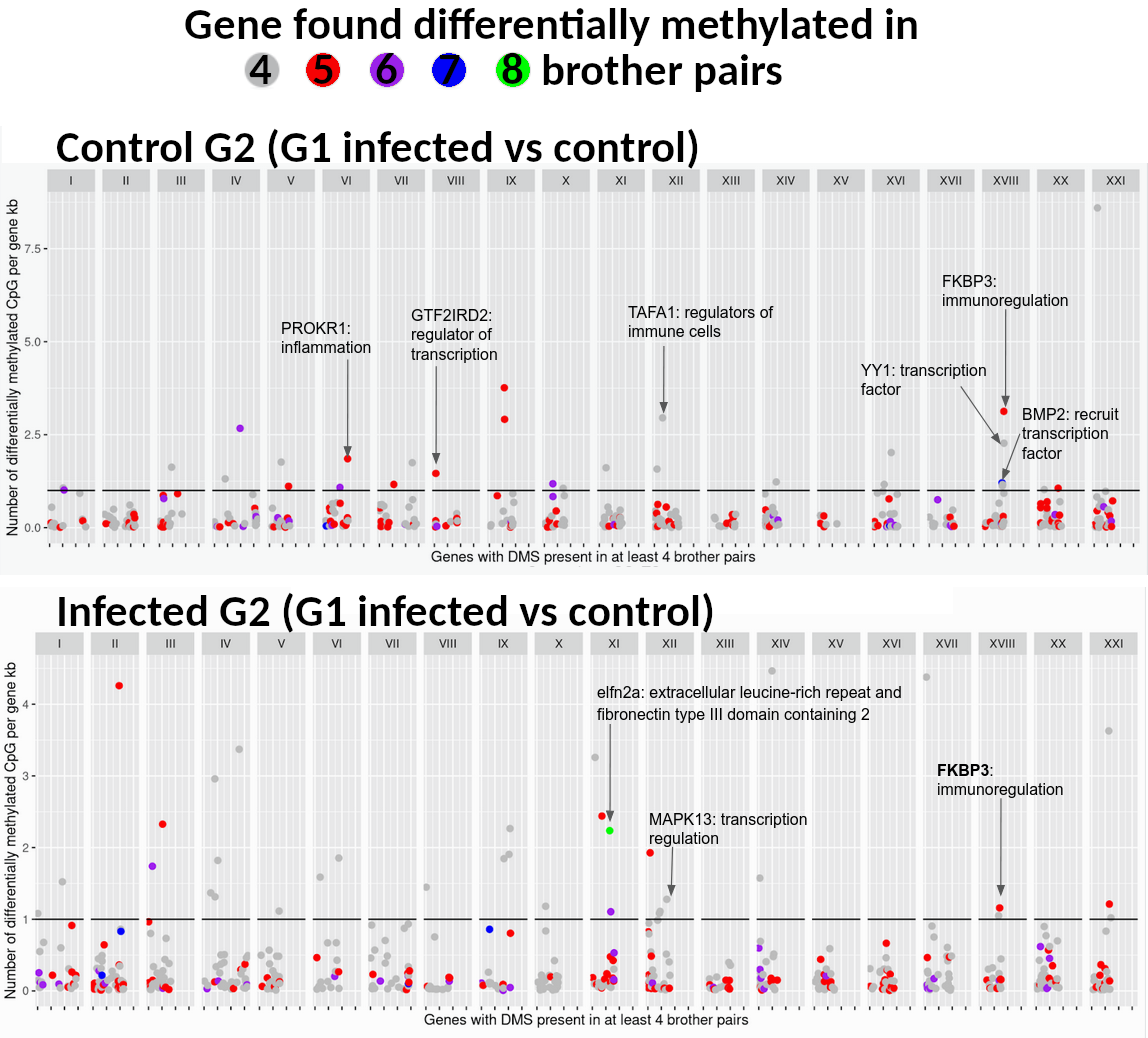
\includegraphics[scale=3]{fig/DMS.png}}

% ----------
% REFERENCES
% ----------
\colorlet{blockbodybgcolor}{white} %back to white
  \block{}{
\textsuperscript{1}Kaufmann, J., Lenz, T. L., Milinski, M., \& Eizaguirre, C. (2014). Experimental parasite infection reveals costs and benefits of paternal effects. Ecology Letters; \textsuperscript{2}Sagonas, K., Meyer, B. S., Kaufmann, J., Lenz, T. L., Häsler, R., \& Eizaguirre, C. (2020). Experimental parasite infection causes genome-wide changes in DNA methylation. Molecular Biology and Evolution; \textsuperscript{3}Thornburn et al., in prep.
  }
\colorlet{blockbodybgcolor}{mylightblue} %back to default


\column{0.44}

% -------------------------
% RESULTS 4
% -------------------------
\block{4. Body condition correlates with methylation at certain positions, in different directions depending on the paternal treatment}{
\Large \centering 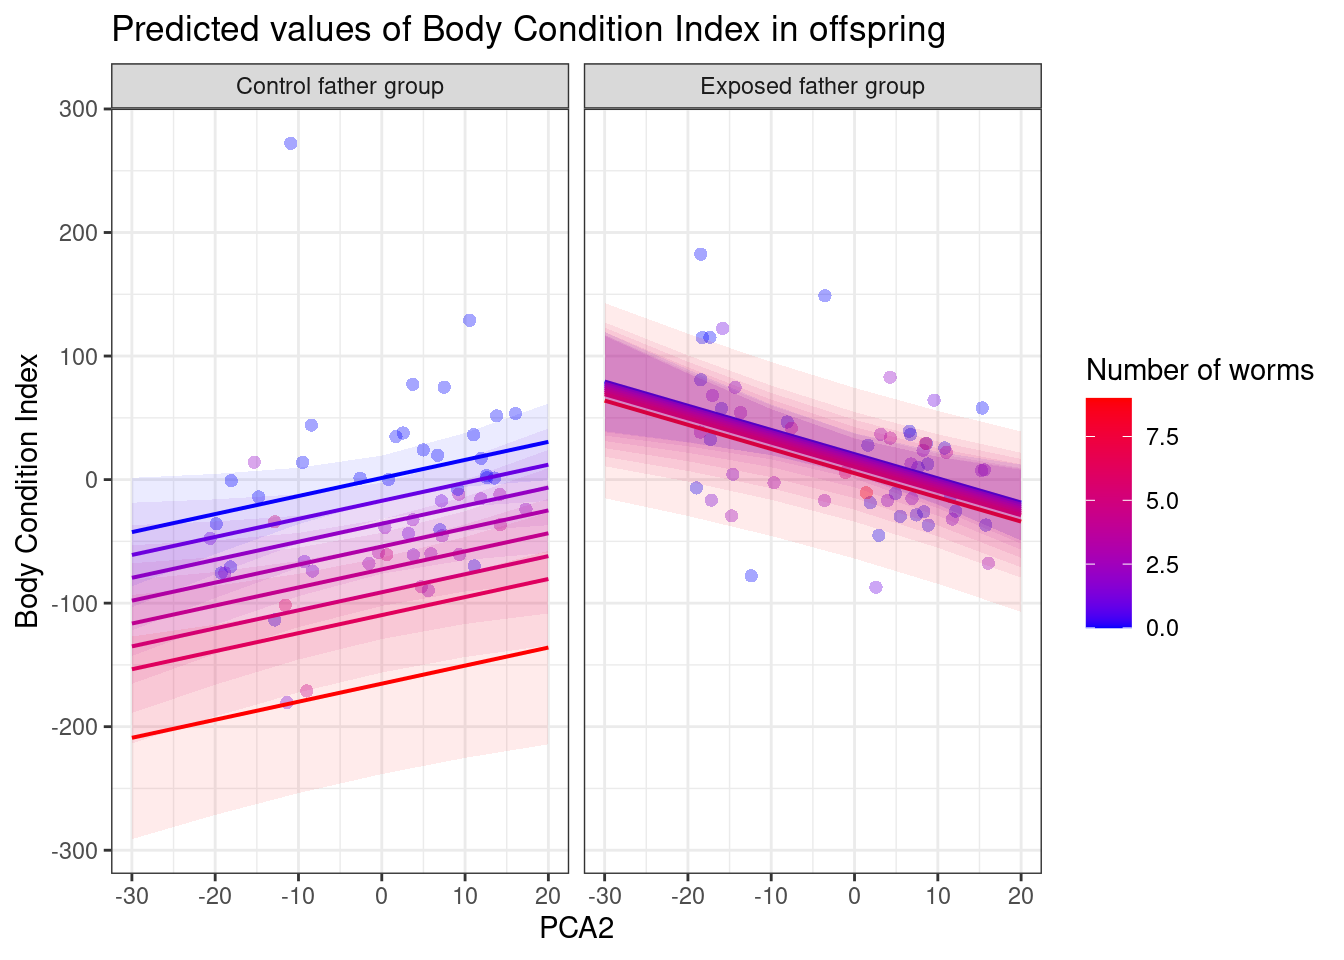
\includegraphics[scale=1.8]{fig/methPheno.png}
}

% ----------
% FUNDING
% ----------
\colorlet{blockbodybgcolor}{white} %back to white
   \block[]{}{\LARGE \centering %\vspace{-3ex}
    
\includegraphics[scale=4.5]{fig/logo--en.pdf}
   }
\colorlet{blockbodybgcolor}{mylightblue} %back to default

\end{columns}

% % ----------------
\end{document}
\endinput
%%
%% End of file
